\chapter{Background and Theoretical Foundation}
\label{ch:background}

This chapter establishes the theoretical and technical foundation necessary to understand the proposed \qos scheduling system. We begin with fundamental \qos concepts, then examine Android networking architecture, traffic classification techniques, and scheduling algorithms.

\section{Quality of Service Fundamentals}
\label{sec:qos-fundamentals}

\subsection{QoS Metrics and Requirements}

Quality of Service refers to the capability of a network to provide differential treatment to different traffic flows, ensuring that critical applications receive adequate resources even under congestion. The primary \qos metrics are:

\begin{definition}[QoS Performance Metrics]
For a traffic flow $f$ traversing a network path, the key performance indicators are:
\begin{itemize}
    \item \textbf{Throughput} $\theta(f)$: The rate of successful data delivery, measured in bits per second (bps)
    \item \textbf{Latency} $\lambda(f)$: The end-to-end packet delay, measured in milliseconds (ms)
    \item \textbf{Jitter} $\sigma_\lambda(f)$: The variance in packet inter-arrival times, $\sigma_\lambda = \sqrt{\mathbb{E}[(\lambda_i - \bar{\lambda})^2]}$
    \item \textbf{Packet Loss Rate} $\rho(f)$: The fraction of packets dropped, $\rho = \frac{packets\_lost}{packets\_sent}$
\end{itemize}
\end{definition}

Different application classes have distinct \qos requirements, as summarized in Table~\ref{tab:qos-requirements}.

\begin{table}[htbp]
\centering
\caption{QoS Requirements by Application Class}
\label{tab:qos-requirements}
\begin{tabular}{@{}lcccc@{}}
\toprule
\textbf{Application} & \textbf{Throughput} & \textbf{Latency} & \textbf{Jitter} & \textbf{Loss} \\
\midrule
VoIP & 64–128 kbps & $<$ 150 ms & $<$ 30 ms & $<$ 1\% \\
Video Conferencing & 0.5–2 Mbps & $<$ 200 ms & $<$ 50 ms & $<$ 2\% \\
Online Gaming & 50–200 kbps & $<$ 50 ms & $<$ 20 ms & $<$ 0.5\% \\
Web Browsing & Variable & $<$ 1 s & Tolerant & $<$ 5\% \\
Video Streaming & 1–10 Mbps & $<$ 5 s & Tolerant & $<$ 1\% \\
File Transfer & Variable & Tolerant & Tolerant & $<$ 0.1\% \\
\bottomrule
\end{tabular}
\end{table}

\subsection{QoS Architectures}

Two primary architectural paradigms have dominated \qos research:

\subsubsection{Integrated Services (IntServ)}

The Integrated Services architecture \cite{rfc2205} employs per-flow resource reservation using the Resource Reservation Protocol (RSVP). Each flow explicitly signals its \qos requirements to network routers, which maintain per-flow state and perform admission control.

\textbf{Advantages:} Provides strong \qos guarantees through explicit resource allocation.

\textbf{Disadvantages:} Poor scalability due to per-flow state maintenance; requires RSVP support across all network hops; complex signaling overhead.

\subsubsection{Differentiated Services (DiffServ)}

The Differentiated Services architecture \cite{rfc2475} employs class-based traffic aggregation. Packets are marked with a Differentiated Services Code Point (DSCP) in the IP header, and routers apply per-hop behaviors (PHBs) based on these markings.

\textbf{Advantages:} Scalable (no per-flow state); simple router implementation; backward compatible.

\textbf{Disadvantages:} Weaker \qos guarantees (statistical rather than deterministic); requires cooperation across administrative domains; end-to-end DSCP marking often stripped by ISPs.

\subsection{Mobile Network QoS Challenges}

Mobile networks introduce unique \qos challenges:

\begin{itemize}[leftmargin=*]
    \item \textbf{Variable Bandwidth:} Cellular link capacity fluctuates due to signal strength, interference, and mobility.
    \item \textbf{Asymmetric Links:} Uplink bandwidth is typically 5–10× lower than downlink, creating severe bottlenecks.
    \item \textbf{Shared Medium:} Multiple users compete for the same cell tower resources.
    \item \textbf{Limited Control:} End-user devices have no control over carrier network \qos policies.
\end{itemize}

Personal mobile hotspots compound these challenges by introducing an additional layer of resource contention among tethered devices.

\section{Android Networking Architecture}
\label{sec:android-networking}

\subsection{Android Network Stack Overview}

The Android network stack is a modified Linux kernel with userspace frameworks for application-level networking. Figure~\ref{fig:android-network-stack} illustrates the layered architecture.

\begin{figure}[htbp]
\centering
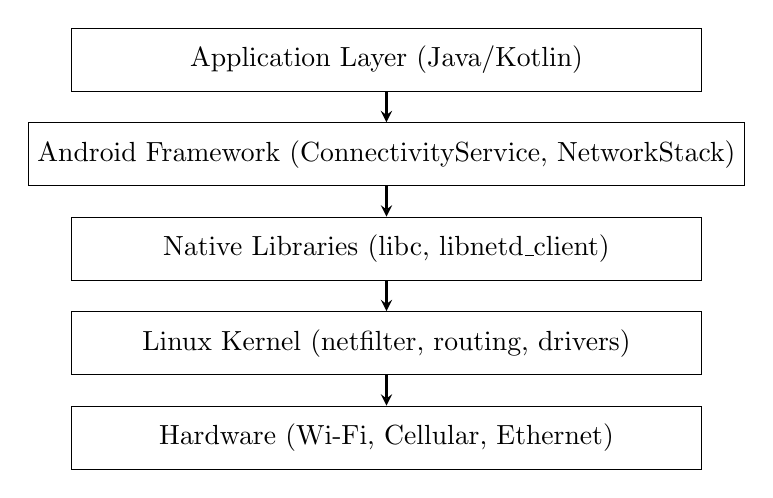
\begin{tikzpicture}[
    box/.style={rectangle, draw, minimum width=8cm, minimum height=0.8cm, align=center},
    arrow/.style={->, >=stealth, thick}
]
    \node[box] (app) at (0,0) {Application Layer (Java/Kotlin)};
    \node[box] (framework) at (0,-1.2) {Android Framework (ConnectivityService, NetworkStack)};
    \node[box] (native) at (0,-2.4) {Native Libraries (libc, libnetd\_client)};
    \node[box] (kernel) at (0,-3.6) {Linux Kernel (netfilter, routing, drivers)};
    \node[box] (hardware) at (0,-4.8) {Hardware (Wi-Fi, Cellular, Ethernet)};
    
    \draw[arrow] (app) -- (framework);
    \draw[arrow] (framework) -- (native);
    \draw[arrow] (native) -- (kernel);
    \draw[arrow] (kernel) -- (hardware);
\end{tikzpicture}
\caption{Android Network Stack Layers}
\label{fig:android-network-stack}
\end{figure}

\subsection{VpnService API}

The \code{android.net.VpnService} class, introduced in Android 4.0 (API 14), enables applications to implement VPN clients without root privileges. The key mechanism is the creation of a TUN (network tunnel) virtual interface.

\subsubsection{TUN Interface Mechanics}

A TUN interface operates at Layer 3 (IP layer), presenting a file descriptor to userspace applications. The kernel routes packets destined for the VPN through this interface, where they can be read, processed, and written back.

\begin{algorithm}[htbp]
\caption{VpnService Packet Processing Loop}
\label{alg:vpn-loop}
\begin{algorithmic}[1]
\Procedure{PacketLoop}{$tunFd$}
    \State $buffer \gets$ allocate(32767 bytes) \Comment{Maximum IP packet size}
    \While{service is active}
        \State $length \gets$ read($tunFd$, $buffer$)
        \If{$length > 0$}
            \State $packet \gets$ parse($buffer$, $length$)
            \State $allowed \gets$ processPacket($packet$)
            \If{$allowed$}
                \State write($tunFd$, $packet.bytes$)
            \EndIf
        \EndIf
    \EndWhile
\EndProcedure
\end{algorithmic}
\end{algorithm}

\subsubsection{VpnService Builder API}

The \code{VpnService.Builder} class configures the TUN interface:

\begin{lstlisting}[language=Java, caption={VpnService Configuration}, label={lst:vpn-builder}]
VpnService.Builder builder = new VpnService.Builder();
ParcelFileDescriptor tunInterface = builder
    .setSession("QoS Scheduler")
    .addAddress("10.0.0.1", 32)      // Virtual IP
    .addRoute("0.0.0.0", 0)          // Route all traffic
    .setMtu(1500)                     // Maximum Transmission Unit
    .establish();
\end{lstlisting}

The \code{addRoute("0.0.0.0", 0)} directive instructs the kernel to route \emph{all} IP traffic through the TUN interface, enabling complete packet interception.

\subsection{Mobile Hotspot Architecture}

Android's mobile hotspot functionality (also called "tethering") is implemented via the \code{TetheringManager} system service. When hotspot mode is enabled:

\begin{enumerate}
    \item A software access point (SoftAP) is created on the Wi-Fi interface
    \item A DHCP server assigns IP addresses to connected clients (typically in the 192.168.43.0/24 subnet)
    \item Network Address Translation (NAT) is configured via \code{iptables} to forward client traffic to the cellular interface
    \item IP forwarding is enabled in the kernel (\code{/proc/sys/net/ipv4/ip\_forward})
\end{enumerate}

Critically, the hotspot operates as a simple Layer 2 bridge with no traffic differentiation. All client packets are forwarded indiscriminately to the uplink interface.

\section{Traffic Classification Techniques}
\label{sec:traffic-classification}

Traffic classification is the process of categorizing network flows into application types. Three primary approaches exist:

\subsection{Port-Based Classification}

Port-based classification uses well-known port numbers assigned by IANA (Internet Assigned Numbers Authority). For example:
\begin{itemize}
    \item TCP port 80: HTTP
    \item TCP port 443: HTTPS
    \item UDP port 53: DNS
    \item UDP ports 16384–32767: RTP (Real-Time Protocol)
\end{itemize}

\textbf{Advantages:} Extremely fast (single hash table lookup); no payload inspection required; works on encrypted traffic.

\textbf{Limitations:} Ineffective for applications using dynamic ports or port obfuscation; cannot distinguish between different applications using the same port (e.g., all HTTPS traffic appears identical).

\subsection{Deep Packet Inspection (DPI)}

DPI analyzes packet payload content to identify application signatures. For example, HTTP traffic can be classified by inspecting the \code{User-Agent} header or URL patterns.

\textbf{Advantages:} High accuracy; can identify specific applications and protocols.

\textbf{Limitations:} Computationally expensive; ineffective on encrypted traffic (TLS/SSL); raises privacy concerns; requires continuous signature database updates.

\subsection{Machine Learning-Based Classification}

ML approaches use statistical features (packet sizes, inter-arrival times, flow duration) to train classifiers (decision trees, neural networks, SVMs) that predict application types.

\textbf{Advantages:} Can classify encrypted traffic; adapts to new applications.

\textbf{Limitations:} Requires labeled training data; high computational overhead; accuracy degrades with concept drift.

\subsection{Hybrid Approaches: DPI-Lite}

DPI-lite combines port-based classification with lightweight heuristics (e.g., packet size distributions, flow duration) to improve accuracy without full payload inspection. This approach is well-suited for resource-constrained mobile environments.

\section{Scheduling Algorithms}
\label{sec:scheduling-algorithms}

\subsection{Token Bucket Algorithm}

The token bucket is a widely used rate-limiting algorithm that controls both average rate and burst size.

\begin{definition}[Token Bucket]
A token bucket $B$ is characterized by:
\begin{itemize}
    \item $r$: Token refill rate (tokens/second)
    \item $b$: Bucket capacity (maximum tokens)
    \item $\tau(t)$: Current token count at time $t$
\end{itemize}

Token refill follows:
\begin{equation}
\tau(t) = \min\left(b, \tau(t_0) + r \cdot (t - t_0)\right)
\end{equation}

A packet of size $s$ bytes is transmitted if $\tau(t) \geq s$, after which $\tau(t) \gets \tau(t) - s$.
\end{definition}

\textbf{Properties:}
\begin{itemize}
    \item Average rate is bounded by $r$
    \item Burst size is bounded by $b$
    \item Smooth traffic shaping without hard rate limits
\end{itemize}

\subsection{Weighted Fair Queuing (WFQ)}

WFQ allocates bandwidth proportional to assigned weights.

\begin{definition}[Weighted Fair Queuing]
Given $n$ flows with weights $w_1, w_2, \ldots, w_n$ and total capacity $C$, the bandwidth allocated to flow $i$ is:
\begin{equation}
B_i = C \cdot \frac{w_i}{\sum_{j=1}^{n} w_j}
\end{equation}
\end{definition}

In our system, we assign weights based on priority classes:
\begin{itemize}
    \item HIGH priority: $w = 4$
    \item MEDIUM priority: $w = 2$
    \item LOW priority: $w = 1$
\end{itemize}

\subsection{Priority Queuing}

Strict priority queuing serves higher-priority queues before lower-priority queues. While simple, it can lead to starvation of low-priority traffic.

\textbf{Our Approach:} We combine token bucket rate limiting with weighted fair queuing to provide both priority differentiation and starvation prevention.

\section{Related Packet Processing Frameworks}
\label{sec:packet-processing}

\subsection{Java NIO for Packet Parsing}

Java New I/O (NIO) provides efficient buffer management via \code{ByteBuffer}, enabling zero-copy packet parsing.

\begin{lstlisting}[language=Java, caption={IPv4 Header Parsing with ByteBuffer}, label={lst:ipv4-parse}]
ByteBuffer buffer = ByteBuffer.wrap(packetBytes);
int versionIhl = buffer.get(0) & 0xFF;
int version = versionIhl >> 4;
int ihl = (versionIhl & 0x0F) * 4;  // Header length in bytes
int protocol = buffer.get(9) & 0xFF;
int srcIp = buffer.getInt(12);
int dstIp = buffer.getInt(16);
\end{lstlisting}

\subsection{Concurrency Considerations}

Packet processing must be thread-safe and efficient. We employ:
\begin{itemize}
    \item \code{ConcurrentHashMap} for device registry (lock-free reads)
    \item \code{@Synchronized} methods for token bucket operations
    \item Kotlin Coroutines for asynchronous I/O
\end{itemize}

\section{Summary}

This chapter established the theoretical foundation for our \qos scheduler:
\begin{itemize}
    \item \qos metrics and requirements for different application classes
    \item Android \vpn Service architecture and TUN interface mechanics
    \item Traffic classification approaches, with port-based classification as the optimal choice for mobile environments
    \item Token bucket and weighted fair queuing algorithms for bandwidth enforcement
\end{itemize}

The next chapter surveys related work in mobile \qos and positions our contribution within the existing literature.
